\subsection{Klassifizierung von Signalen S.7}
\begin{table}[H]
	\begin{tabularx}{\textwidth}{|X|X|}
		\hline
		\begin{minipage}{\linewidth}Energiesignal $E=\int_{-\infty}^{\infty}|x(t)|^2 dt < \infty$ \end{minipage}
		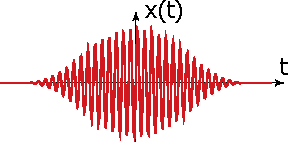
\includegraphics{content/03_Signale/energiesignal.pdf}
		& 
		\begin{minipage}{\linewidth}Leistungssignal $ P=\lim\limits_{T->\infty} \frac{1}{T} \int_{-T/2}^{T/2}|x(t)|^2 dt < \infty$\end{minipage}
		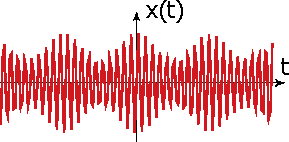
\includegraphics{content/03_Signale/leistungssignal.pdf}
		\\
		\hline
		\\
		\begin{minipage}{\linewidth}aperiodisches Signal $x(t) \neq x(t+n \cdot T)$\end{minipage}
		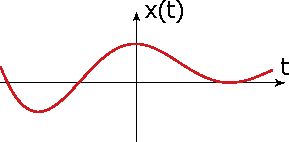
\includegraphics{content/03_Signale/aperiodischessignal.pdf}
		& 
		\begin{minipage}{\linewidth}periodisches Signal$x(t) = x(t+n \cdot T)$\end{minipage}
		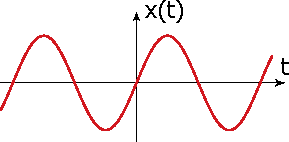
\includegraphics{content/03_Signale/periodischessignal.pdf}
		\\
		\hline
		\\
		\begin{minipage}{\linewidth} deterministisches Signal \\ $x(t) = f(t)$ Verlauf ist bekannt \end{minipage}
		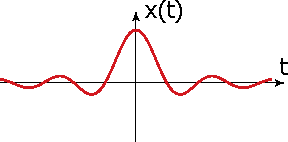
\includegraphics{content/03_Signale/deterministischessignal.pdf}
		&
		\begin{minipage}{\linewidth}{stochastisches Signal: Signalverlauf ist unbekannt bzw. zufällig}\end{minipage}
		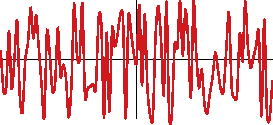
\includegraphics{content/03_Signale/stochastischessignal.pdf}
		\\
		\hline
		\\
		\begin{minipage}{\linewidth} zeitkontinuierliches Signal $x(t)$ ist immer definiert \end{minipage}
		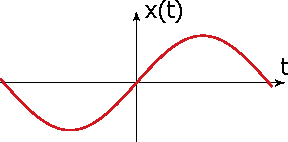
\includegraphics{content/03_Signale/zeitkontinuierlichessignal.pdf}
		&
		\begin{minipage}{\linewidth}zeitdiskretes Signal $x(t)$ ist nur an diskreten Punkten definiert\end{minipage}
		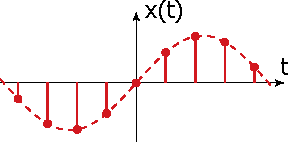
\includegraphics{content/03_Signale/zeitdiskretessignal.pdf}
		\\
		\hline
		\\
		\begin{minipage}{\linewidth}amplitudenkontinuierliches Signal\end{minipage}
		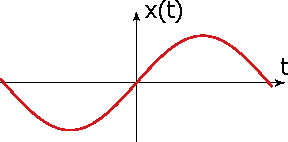
\includegraphics{content/03_Signale/amplitudenkontinuierlichessignal.pdf}
		&\begin{minipage}{\linewidth} quantisiertes Signal \end{minipage}
		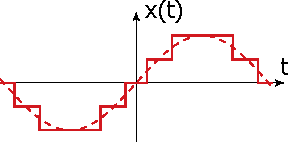
\includegraphics{content/03_Signale/quantisiertessignal.pdf}
		\\
		\hline
		\\
		\begin{minipage}{\linewidth} Zeit- und Amplitudenkontinuierliches Signal (Analog) \end{minipage}
		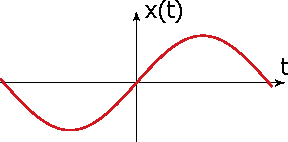
\includegraphics{content/03_Signale/zeitamplitudenkontinuierlichessignal.pdf}
		& \begin{minipage}{\linewidth} Zeitdiskret und Quantisiert \end{minipage}
		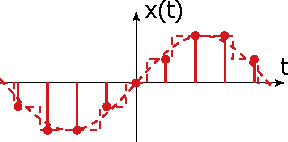
\includegraphics{content/03_Signale/zeitdiskretquantisiert.pdf}
		\\
		\hline
	\end{tabularx}
\end{table}
\newpage